%
% 1.2
%
\section{Coursework}%

\newthought{The approach to social science} that we follow in this course is driven by a dual logic of inquiry: we start with the description of quantitative data, and we end with its analysis through statistical models. The procedures involved in this process are computational and require some technical knowledge of computers and mathematics.%
	%
	%

	%%% They’re someone who can ask and answer questions about and with data.
	%%% http://www.analyticstory.com/hadley-wickham/

	%%% I A key principle in applied statistics is that you should be able to connect between the raw data, your model, your methods, and your conclusions

	%%%%Controlled experiments are the gold standard, but I never do them!

%%% I (Some) computer scientists' view: we don't need controlled experiments; we can automatically learn from observational data

%%% I Psychologists' view: each causal question requires its own experiment

%%% I Observational scientist's version: each causal question requires its own data analysis

%%% Sample surveys (for the problem of extending from sample to population)

%%% Descriptive observational research (for the problem of modeling complex interactions and response surfaces)

%%%Political science is largely an empirical discipline. That is, most of us studying politics do so because we are motivated by real world political events, either historical, current, or even events yet to happen. We want to know why these events happen and how to make sense of them. Political science trys to answer these questions in a rigorous way. Data analysis is thus a critical component of political science, serving two important purposes: (1) providing numerical descriptions or summaries of political phenomena, facilitating comparisons across time, countries, states, people, etc; (2) testing theories, models and hypothesis about politics.


% All this is to say that this class involves a little math. Or, as I like to put it, this class is ‘‘techie for fuzzies’’: an introduction to the way political scientists use the tools of statistics to rigorously understand political events. I assume virtually zero mathematical background on your part, either because you didn’t take math in high school or because you’ve forgotten it. I assume no prior background with using computers for data analysis. The classes will have a heavy ‘‘show-and-tell’’ feel to them, where I will use statistical software to do data analysis.

%%%forecast the effects of interventions, the trajectory of existing trends, and the likely strategies

%%% http://understandingsociety.blogspot.fr/2009/01/predictions.html

% 1.2.1
%
\subsection{Course outline}%
  \index{Course!Outline and readings}
	%
	%

\newthought{This course} follows the standard regulations of Sciences Po, \ie, attendance is compulsory, every class comes with homework and readings, and plagiarism on any element of coursework is strongly sanctioned. Please turn to your academic regulations for more details on any of these topics.%

The course itself is organised in twelve two-hour sessions that run over a single semester. Its content is structured around three teaching goals:%

\begin{enumerate}
  
  % 1. Statistics

	\label{sec:textbooks}%
	\index{Course!Readings}%
  \item The course covers some \textbf{essential aspects of statistical analysis}, from describing variables to running regression models.%
  
  This learning objective requires that you read from textbooks that apply fundamental statistical theory to social science research. The primary textbook for this course is \citetitle{Urdan:2010a}\footcite{Urdan:2010a}, one of the shortest and most effective introduction to the course topics. %
	
	Towards the end of the class, we turn to \citetitle{FeinsteinThomas:2002d}\footcite{FeinsteinThomas:2002d}, a clearly worded introduction to quantitative methods for qualitatively-minded social scientists, for additional clarifications on regression modelling.%
  
	\index{Course!Syllabus}%
  Both textbooks appear in the course syllabus%
		\footnote{\url{https://github.com/briatte/srqm/blob/master/course/syllabus.pdf?raw=true}} %
    as well as in the final bibliography of this document. Please read the course syllabus in full at that stage, and copy the reading schedule to your agenda.%
		
  The textbook readings for this course will give you a more detailed view of statistics than this guide can provide. Furthermore, since the course slides are mostly trivia taken from the course blog,%
  \footnote{\url{http://srqm.tumblr.com/}} %
    you really have no other choice than to take the time to go through the assigned readings. The weekly readings appear at the beginning of each section of this guide, in the course syllabus, and on the course website.%

  % 2. Stata

  \item The course also explains \textbf{how to operate Stata} for basic data analysis and visualization.%

    \newthought{There will be one Stata do-file to study per week of class.} We will start looking at the do-file in class, and you will be asked to finish replicating it at home. Some online tutorials and Stata Press handbooks, like the recent one by \citeauthor{Mitchell:2012a} on applied regression,\footcite{Mitchell:2012a} can also be used as additional companions.%
		\footnote{See an indicative list of tutorials and books on the course website and on the course wiki: \url{https://github.com/briatte/srqm/wiki/stata}} %
    
    The do-file for the first week covers basic Stata settings and data exploration commands. It will show you how to start exploring the course datasets. Your weekly mission is to replicate the do-file of the current session. After running through the setup described in Section~\ref{sec:course-setup}, the following command will open the do-file for Week~1:%

      \begin{docspec}
        doedit code/week1.do
      \end{docspec}

     \newthought{Read through the do-file and execute (run) its commands sequentially}, reading the comments that precede each block of code. This practice (replicating the course do-files) will show you how to code various things in Stata, which will become handy when you start writing code for your own research project.%
    
     The baseline advice to survive the computing component of the course is very simple: practice by reading and writing code every week of class. If this is going to be the only time in your student life where you get to write statistical code, make sure that you get the most out of it. There is a fair chance that you will be offered to use that skill one day.%
  %

  % 3. Research

  \index{Course!Research projects!Final paper}%
  \item The course finally works assists students to work in pairs over \textbf{small-scale research projects}, on which the grading for the course is based.%
  
    Each student pair submits two draft versions of their empirical analysis (Stata code) and analytical report (research paper) during the semester, and one final version of their at the end of the class. The steps that each student pair needs to take throughout the semester to complete their research projects can be summarised as follows:%

    \begin{itemize}
      \item \textbf{setting up your computer} to follow the course and access the teaching material from the \SRQM folder (Weeks~1--2; Section~\ref{ch:intro});%
      \item \textbf{registering a research topic} with a student partner from your class in the course projects list (Weeks~2--3);%
      \item \textbf{exploring the course datasets} to find variables related to your research topic and select some variables of interest (Weeks~3--4; Section~\ref{ch:data});%
      \item \textbf{submitting your first draft} that presents the topic, the data the distributions of the variables under scrutiny (Weeks~4--5; Section~\ref{ch:distr});%
      \item \textbf{revising your draft} and resubmitting it with additional significance tests of associations in the data (Weeks~5--8; Sections~\ref{ch:asso} and \ref{ch:ols}); and%
      \item \textbf{submitting your final paper} in which you model your data with linear or logistic regression (Weeks~9--12; Sections~\ref{ch:lin} and \ref{ch:log}).%
    \end{itemize}

    \newthought{The deadline} for the first draft is generally set to mid-term (Week~5). The deadline for the revised draft is generally set to Week~10. The deadline for the final paper is generally set to the last course session. In order to make all groups benefit from the challenges that arise in each project, you will be offered to submit questions to collective FAQs before every deadline.%
    %

    \hlred{Exact deadlines and all other project instructions are covered exclusively in class, which is why you should \textbf{attend every week and catch up if absent}.} The course sessions are cumulative: you cannot just skip one as if it had never happened. Your stress and workload \emph{will} increase if you skip a week with the hope of catching up later, and you will \emph{not} be able to fix your project if you let it rest.%
    %

		\newthought{Please read} \citeauthor{White:2005a}'s \citetitle{White:2005a}%
      \footcite{White:2005a} %
      for a refresher on how to write an empirical research paper. If you have never carried empirical research before, please also turn to \citeauthor{BoothWilliams:2003v}'s \citetitle{BoothWilliams:2003v}%
      \footcite{BoothWilliams:2003v} %
      for a detailed explanation on how to prepare a research project. All other teaching material for the research projects paper templates and example papers, is distributed through Google Drive in class.%
    % ^^^^^^^ 
    % replace by internal Google Documents support at Sciences Po (2013)?

		You are encouraged to use your research paper for other purposes than this course: think of it as work that you will be able to add to your student portfolio. Some students have used the coursework from this class to draft \textsc{Msc} dissertations, working papers or essays from other classes on research design and research methodology. Other students have used Stata for other projects in organizations that either consume or produce data.%
      \footnote{Examples from past years include a lot of consulting work on urban areas, research on land law and its effects on economic development, and estimating the number of refugees in a given geographical area to help plan the work of a nongovernmental organization.}%
		%
    
\end{enumerate}

% 1.2.2
%
\subsection{Course setup}%
	%
	%
	\label{sec:course-setup}%
	\index{Course!Setup}%
	%
	%

	\newthought{This section} explains how to set up Stata to follow the course. It assumes very little knowledge of computers or Stata, but please make sure that you have read through the previous section first. \hlred{\textbf{Make sure that you successfully set up your computer} for the course, and that you know how to run the setup again if needed.}%

	The setup below has been tested on Sciences Po workstations equipped with Stata~11. You might run into issues with this setup only if you use a computer with heavy user restrictions or with a really old copy of Stata. Please let us know if the setup fails.%
    \footnote{GitHub users can report issues on the course repository: \url{https://github.com/briatte/srqm/issues}}%
	
	% i
	%
	\paragraph{Get the teaching material}%
		\label{sec:teaching-pack}%
		\index{Course!Teaching material}

	\newthought{The `Teaching Pack' for this course comes in a single folder,} called the \SRQM folder, which you will have to access very frequently inside and outside class. Download and unzip the folder from its webpage%
		\footnote{\url{http://f.briatte.org/srqm/}} %
		or use the copy provided in class, and keep the \ZIP archive of the folder as a backup.%
		
	\hlred{Move the \SRQM folder to a \textbf{stable location} that you can easily locate on your hard drive, and keep it at that same location throughout the entire course.} Most users deal with this requirement by putting the \SRQM folder with the rest of their study files and then creating an alias to it on their Desktop.%
	
	Use any method that does not involve clicking for two full minutes to access the \SRQM folder, and do not rename its enclosing folders. For simplicity, leave the folder name to \SRQM for the class, and rename it to whatever you like at the end of the semester.%
	
	At that stage, \textbf{check the contents} of the \SRQM folder. The \SRQM folder contains the entire course material, minus the copyrighted textbooks and Stata software. The full contents of that folder, shown in Figure~\ref{fig:srqm-folder}, must stay available on your hard drive during the entire course.%
		%
		%

		\begin{figure}%
		  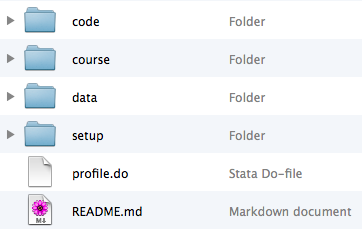
\includegraphics[width=\textwidth]{srqm-folder}
      
		  \caption{The contents of the \SRQM folder should match %
			this screenshot from a \OSX setup.}
		    \label{fig:srqm-folder}
		\end{figure}
		%
		%
		
	The \course folder contains the course slides and syllabus, as well as this guide. The \data folder contains a selection teaching datasets, and the \code folder will host the course do-files (covered below at p.~\pageref{sec:do-files}). The \setup folder and \filename{profile.do} files provide additional course functionalities. All folders are required for the course to roll out properly.%
		%
		%	\index{Computers!File and folder paths}%

	\index{Computers!URLs}%
	You need to understand the file structure of the course to understand how Stata will locate its files and folders from their \textbf{paths}. The path to the \SRQM folder, for example, might look like this on \OSX:\\[1em]%
	
	\begin{docspec}
		/Users/fr/Documents/Teaching/SRQM
	\end{docspec}
	
	The beginning of that path is often abbreviated through a tilde, so that \texttt{~/} designates the user folder. Stata understands that `tilde expansion' notation. Stata for Windows also understand paths with \texttt{\textbackslash} backslashes slashes as used in Windows, where the path generally starts on the \texttt{C:} drive:%

	\begin{docspec}
		C:\textbackslash{}Users\textbackslash{}Ivo\textbackslash{}Desktop\textbackslash{}SRQM
	\end{docspec}
	
	Once a folder has been set as the \emph{working directory}, Stata can locate files and folders from within it by using relative paths. The example below shows the relative path of the \texttt{nhis9711.dta} dataset in the \texttt{\data} folder:\\[1em]%
	
	\begin{docspec}
		/Users/fr/Documents/Teaching/SRQM/\hlred{\underline{data/nhis9711.dta}}
	\end{docspec}

	File paths are used in Stata to open and save datasets and other types of files. In some cases, it is also possible to open files from online sources by specifying their \URL. A \URL is an Internet address like the one that brings up the course webpage.%
		\footnote{\url{http://f.briatte.org/teaching/quanti/}}%
		%
		%
	
	We will use file paths and \URL\ s extensively throughout the course, so make sure that you understand both. I do my best to keep things tidy on my end by using Internet shortlinks and simple, informative folder and file names for the course material. You will have to do the same on your end.%
		%
		\footnote{For instance, you will be required to submit your work under a specific group name that includes your family names in alphabetical order.}%
		%
		%

	% ii
	%
	\paragraph{Set your working directory}%
		\label{sec:working-directory}%
		\index{Course!Teaching material}

  \newthought{Open Stata.} \OSX users can simply double-click the application icon. \hlred{\textbf{Windows users} will have to run Stata with administrator privileges: do this by right-clicking the Stata application icon then selecting `Run as Administrator.'} This will allow Stata to save files anywhere on the hard drive, which is required only for this setup.%
	 
	You are now going to set the working directory, which is the folder in which Stata opens and saves files by default. From the `File' menu, choose `Change working directory...', then select the \SRQM folder and press \texttt{Enter}. You will see something like the following printed in the Results window, that is, a folder path ending with the \SRQM folder:\\[1em]%
	
		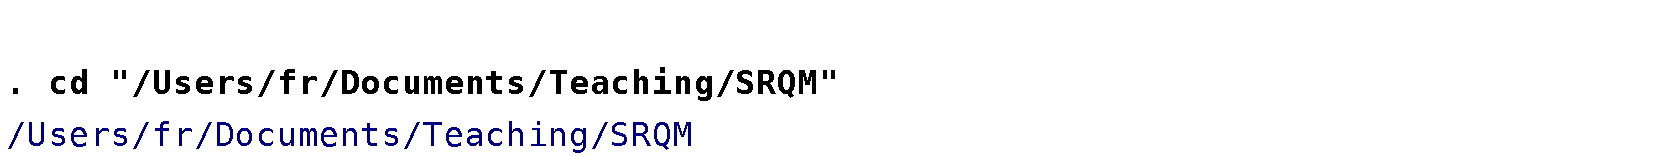
\includegraphics{srqm-cd}\\[1em]

	As the code output shows, the Stata command to do what you did through the `File' menu is \cmd{cd}, for `\underline{c}hoose \underline{d}irectory,' followed by the path to the desired folder. Now that you have learnt a Stata command, try it out by typing the following lines in the Command window and pressing \texttt{Enter} to execute each line:%
	
	\begin{docspec}
		cd ..\\
		cd SRQM
	\end{docspec}
	
	The first command, \texttt{cd ..}, changes the working directory to the enclosing folder, which in my case is the \texttt{Teaching} folder. The second command returns to the \SRQM folder and makes it the working directory again:\\[1em]%
		
	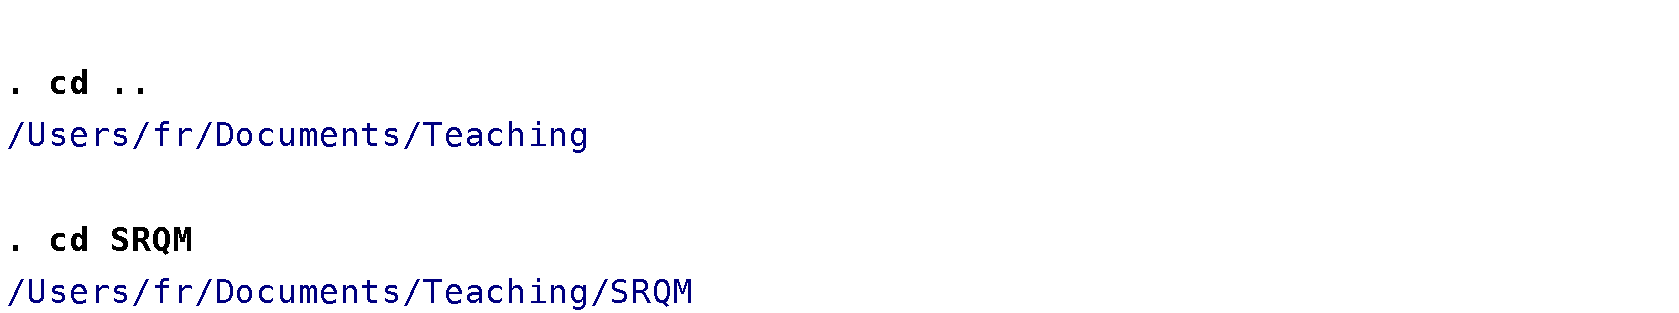
\includegraphics{srqm-cd-back}\\[1em]
	
	You can also list the contents of the working directory with the \cmd{ls} command. The example below will show the full contents of the \SRQM folder with detailed file information:%
	
		\begin{docspec}
			ls
		\end{docspec}

		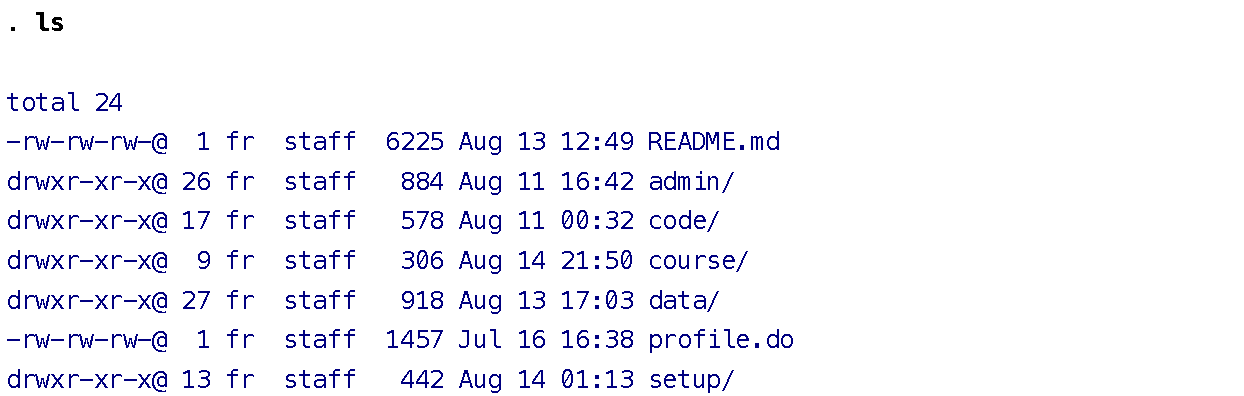
\includegraphics{srqm-ls}\\[1em]
			
	The \cmd{ls} command below will produce a more focused output by listing only the files located in the \data folder that end with the \ext{.dta} extension, which is the Stata dataset format (Figure~\ref{fig:stata-dta-icon}):%

		\begin{marginfigure}
			
\includegraphics[width=.66\textwidth]{stata-dta-icon}
			\caption{Stata~12 dataset icon.}
			\label{fig:stata-dta-icon}
		\end{marginfigure}

		\begin{docspec}
			ls data/*.dta, w
		\end{docspec}
			 
	The command will list the teaching datasets used in the course, showing only their filenames because you passed the \coab{wide}{w}{ls} option to it:\\[1em]%
 
		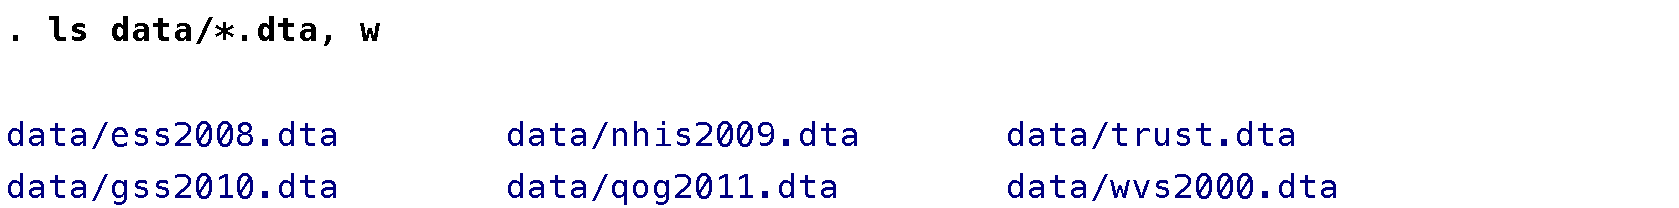
\includegraphics{srqm-ls-dta}\\[1em]
	
	To finish this little exercise with folder navigation from the command line, make sure that your working directory is the \SRQM folder. Use the \cmd{pwd} command to get the path printed once more:%
	
		\begin{docspec}
			pwd
		\end{docspec}
	
	Your working directory should again end with the \SRQM folder, which is what we need to run the course setup in the next section:\\[1em]%
	
		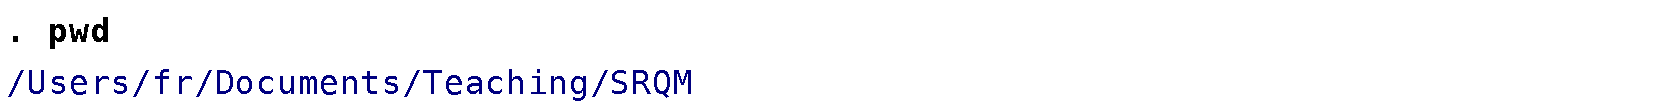
\includegraphics{srqm-pwd}\\[1em]
  
	% iii
  %
  \paragraph{Run the \SRQM setup}%
		\label{sec:setup}%

	To finish setting up your computer for the course, make sure that you are connected to the Internet, then type the following command in the Command window and press \texttt{Enter}:%
		%
		%
		
		\begin{docspec}
			run profile
		\end{docspec}
	
	\hlred{\textbf{Note:} the command will not work if you have not set the \SRQM folder as your working directory}, and that its syntax is a strict one: do not add capital letters, separate the words \texttt{run} and \texttt{profile}, and of course, use the exact spelling.%
	
	This command will trigger a bunch of setup utilities that install the additional Stata commands listed in Table~\ref{tbl:additional-commands}, uncompress the course datasets and adjust some Stata system options.%
		%
		\footnote{For example, the setup adjusts Stata memory on older versions of Stata to deal with some of the larger course datasets. Stata~12 now handles memory automatically.} %
		%
		%
		
	\bigskip

\begin{fullwidth}
	\begin{table}
		\footnotesize
		\begin{tabular}{lll}
		\toprule
		Package & Description \\
		\midrule
		\emph{Installed from the \SSC server:} & & \\
	  \quad \pkg{estout} & export regression results \\
		\quad \pkg{fre} & frequencies with value labels \\
	  \quad \pkg{kountry} & standardised regions and country names\\
	  \quad \pkg{leanout} & simplified regression results\\
		\quad \pkg{lookfor\_all} & search for variables across datasets \\
	  \quad \pkg{mkcorr} & export correlation tables\\
	  \quad \pkg{plotbeta} & regression coefficient plots \\
    % \quad \pkg{qog} & download \QOG data\\
		\quad \pkg{scheme-burd} & graph scheme \\
		\quad \pkg{spineplot} & mosaic plots \\
	  \quad \pkg{spmap} & maps \\
	  \quad \pkg{tab\_chi} & residuals for Chi-squared tests\\
	  \quad \pkg{tabout} & export summary statistics\\
	  \quad \pkg{wbopendata} & download World Bank data\\
		\addlinespace
		\emph{Installed from elsewhere:} & & \\
		\quad \label{install-gstd01}\cmd{gstd01} & standardize a variable to $0$-$1$\\%
    %; used at p.~\pageref{sec:gtsd01} \\
		\quad \label{install-clarify}\pkg{clarify} & simulation\\%
    %; used at p.~\pageref{sec:clarify} \\
    % \quad \pkg{schemes} & graph schemes \\
		\emph{Installed with the course setup:} & & \\
    % \quad \pkg{repl} & replication utility \\
		\quad \cmd{srqm} & course utilities \\
    \quad \cmd{sbar} & plots for categorical data\\
		\quad \cmd{stab} & export summary statistics tables \\
		\bottomrule%\\[1em]
		\end{tabular}
		%
		\caption{Additional commands installed by the course setup.}
		\label{tbl:additional-commands}
	\end{table}
\end{fullwidth}

%
  
	You will get a `\texttt{Hello!}' message when the setup is complete.%
	
  \hlred{\textbf{Note:} if you move or rename the \SRQM folder, the setup will break and you will have to repeat the steps covered in the previous paragraphs to fix the issue:}%
		%
		%	
		\begin{enumerate}
			\item run as administrator (if using Windows),
			\item select the \SRQM folder as the working directory, and
			\item type \texttt{run profile} to go through setup again.
		\end{enumerate}
	  
	The setup overwrites the \filename{profile.do} file of the Stata application folder to redirect it to the \SRQM folder for the time of the course. From there, it runs another \filename{profile.do} file that verifies the integrity of the teaching material and reruns parts of the setup if necessary.%
		%
		%
		
	The setup also loads the \cmd{srqm} teaching utilities, like \cmd{srqm\_get}, which is used in class to download the latest version of the course material from a temporary course server, and \cmd{stab}, which is used to produce \underline{s}imple \underline{tab}les of summary statistics (see its detailed instructions at p.~\pageref{cmd:stab}).%
    %
    %
		
  \newthought{At the end of the course}, delete the \texttt{profile.do} from the Stata application folder to stop automatically setting the \SRQM folder as your working directory. Alternately, run the \texttt{srqm\_link, clean} command to do so and get a `\texttt{Bye}' message. This will let you work with Stata from any other working directory.%
		%
		%

%
%
\subsection{Course datasets}
	\label{sec:data-sources}
	\index{Datasets!Data sources}%
	%
	%

  \newthought{Stata can load example data} with the \cmd{sysuse} and \cmd{webuse} commands, as shown with the \code{lifeexp} dataset at p.~\pageref{lifeexp}. The course provides its own teaching datasets, listed in Table~\ref{tbl:data-sources}. The course setup will also download two files to plot world maps in Stata.%

  \bigskip
\begin{table}
  \begin{center}
  \footnotesize
  \begin{tabular}{lll}
    \toprule
    Filename & Data & Year(s) \\
    \midrule
    \quad \texttt{ess2008}  & \ess  & Round~4, 2008\\
    \quad \texttt{gss0012}  & \gss  & 2000-2012\\
    \quad \texttt{nhis2009} & \nhis & 2000-2009\\
    \quad \texttt{qog2013}  & \qog  & 2009 ± 3 years\\
    \quad \texttt{wvs2000}  & \wvs  & Wave~4, 2000\\
    \bottomrule
  \end{tabular}
  \end{center}
  \label{tbl:data-sources}%
\end{table}


	All course datasets are in the \data folder, from where they can be loaded into memory with the \cmd{use} command. The command requires that you pass the exact file path of the dataset, and that you include quotes if the file path contains spaces. Note that the \cmd{use} command can also copy data from a \URL, which we might quickly review later on.%

  The example below will load a course dataset in memory:%

		\begin{docspec}
			* Load the National Health Interview Survey, years 2000-2009.\\
			use data/nhis9711, clear
		\end{docspec}

  Stata looks for \ext{.dta} files by default, so the file extension can be omitted from the command. The \opt{clear}{use} option ensures that Stata will load the data even if there is already modified data in memory. Because you are never going to overwrite the original datasets, you are never going to lose anything crucial by doing so.%

	Stata can only open one dataset at the time and opens data silently: if the operation succeeds, nothing is printed on screen, except for a short message if the dataset has been labelled by its creator. All datasets for this course are slightly modified versions of the original ones and will print a short message when opened:\\[1em]%
		
		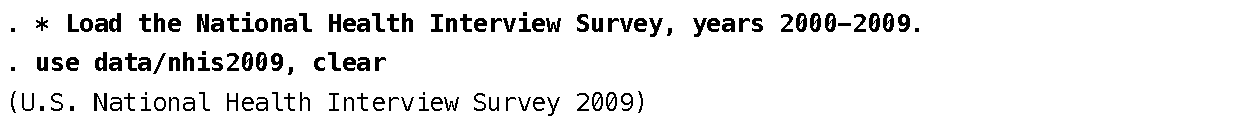
\includegraphics{use-nhis}\\[1em]%

  \newthought{The next paragraphs describe the course datasets}. These are provided in Stata 9/10 \ext{.dta} format on an ``as-is'' basis: please reference their original sources and use them for teaching purposes only. Modifications to the original files are coded in the \texttt{srqm\_data.ado} script, which is part of the course utilities.%
    \footnote{\url{https://github.com/briatte/srqm/wiki/course-utilities}}%
    
  The documentation below shows how to load the datasets in memory from the \SRQM folder with the \cmd{use} command, sometimes with an additional \cmd{if} argument to restrict the data to a particular survey year or round. Further illustrations of how to select a particular segment of your data for analysis are provided in the next sections. You will have to make your own data selection for your research project.%

\paragraph{\ess (\texttt{ess0810})}

The \texttt{ess0810} dataset holds Rounds~4~(2008) and 5~(2010) of the \ess (\ESS).%
	\footnote{\url{http://ess.nsd.uib.no/ess/round4/}}

\begin{quote}
	The \ess (the \ESS) is an academically-driven social survey designed to chart and explain the interaction between Europe's changing institutions and the attitudes, beliefs and behaviour patterns of its diverse populations.%
	\footnote{\url{http://www.europeansocialsurvey.org}}
\end{quote}

Example usage:

\begin{docspec}
  * Load the ESS dataset.\\%
  use data/ess0810, clear\\[1em]%
  %
  * Load latest survey round.\\%
	use data/ess0810 if essround == 4, clear\\[1em]%
  %
  * Load data for one country.\\%
  use data/ess0810 if cntry == "RU"\\[1em]%
  %
  * Load data for two countries.\\%
	use data/ess0810 if inlist(cntry, "CZ", "SK"), clear
\end{docspec}

The \ESS dataset should be used with the following survey weights:

\begin{docspec}
  * Set survey design weights.\\%
	svyset [pw = dweight]
\end{docspec}

See the \ESS weighting guide for details on using additional population weights to use a sample that representative of the European population.%
  \footnote{\url{http://ess.nsd.uib.no/ess/doc/weighting.pdf}} %
  You might also want to take a look at Matthias Ganniger's training module on weigthing the \ESS, which is an excellent five-chapter introduction to the topic.%
  \footnote{\url{http://essedunet.nsd.uib.no/cms/topics/weight/}}

The datasets for both rounds were downloaded from the ESS data server,%
  \footnote{\url{http://nesstar.ess.nsd.uib.no/}} %
  and the codebooks were downloaded from the \ESS data website, on which you can also find a very useful series of booklets that present overall and `topline' results.%
  \footnote{\url{http://ess.nsd.uib.no/}} %
  Check the cumulative dataset for other ESS survey waves,%
  \footnote{\url{http://ess.nsd.uib.no/downloadwizard/}} %
  and refer to the original datasets for nation-specific variables (\eg mother's education in Slovakia or party membership in Belgium).

\paragraph{\gss (\texttt{gss0012})}

The \texttt{gss0012} dataset holds data from the U.S. \gss (\GSS) for years 2000-2012.

\begin{quote}
	The \GSS contains a standard `core' of demographic, behavioral, and attitudinal questions, plus topics of special interest. Many of the core questions have remained unchanged since 1972 to facilitate time-trend studies as well as replication of earlier findings.%
	\footnote{\url{http://www3.norc.org/GSS+Website/}}
\end{quote}

Example usage:

\begin{docspec}
  * Load GSS dataset.\\%
  use data/gss0012, clear\\[1em]%
  %
  * Load latest survey year.\\%
	use data/gss0012 if year == 2012, clear
\end{docspec}

The \GSS dataset should be used with the following survey weights:

\begin{docspec}
  * Set survey design weights.\\%
	svyset vpsu [pw = wtssall], strata(vstrat)
\end{docspec}

% link to Pedlow requires fix
% http://tex.stackexchange.com/questions/12230/getting-percent-sign-into-an-url-in-a-footnote#12233

See Appendix~A of the \GSS codebook%
   \footnote{\url{http://publicdata.norc.org:41000/gss/documents//BOOK/GSS_Codebook_AppendixA.pdf}} %
   and the online technical paper ``Calculating Design-Corrected Standard Errors for the General Social Survey, 1988-2010''%
  \footnote{\url{http://publicdata.norc.org:41000/gss/documents//OTHR/GSS\%20design\%20variables.pdf}} %
   by Steven Pedlow for details, especially if you plan to use older survey years for which the sampling and weighting design are different.%

The data are extracted from the \GSS 1972-2012 cumulative cross-sectional dataset (Release 2, June 2013).%
  \footnote{\url{http://www3.norc.org/GSS+Website/Download/STATA+v8.0+Format/}}

\paragraph{\nhis (\texttt{nhis9711})}

The \texttt{nhis9711} dataset holds sample adult data for years 1997--2011 of the U.S. \nhis (\NHIS).

\begin{quote}
	The \nhis (\NHIS) has monitored the health of the nation since 1957. \NHIS data on a broad range of health topics are collected through personal household interviews. For over 50 years, the U.S. Census Bureau has been the data collection agent for the \NHIS. Survey results have been instrumental in providing data to track health status, health care access, and progress toward achieving national health objectives.%
	\footnote{\url{http://www.cdc.gov/nchs/nhis.htm}} 
\end{quote}

Example usage:

\begin{docspec}
  * Load NHIS dataset.\\%
  use data/nhis9711, clear\\[1em]%
  %
  * Load latest survey year.\\%
	use data/nhis9711 if year == 2011, clear
\end{docspec}

The \NHIS dataset should be used with the following survey weights:

\begin{docspec}
    * Set survey design weights\\
    svyset psu [pw = perweight], strata(strata)
\end{docspec}

See the IHIS/NHIS user notes on variance estimation for more details.%
  \footnote{\url{http://www.ihis.us/ihis/userNotes_variance.shtml}}

The data come from the Integrated Health Interview Series website.%
  \footnote{\url{http://www.ihis.us/}} %
  In the course, we use this dataset to illustrate normality in the distribution of the Body Mass Index in American adults. Our class estimates will slightly differ from the official figures because we will be using the public \nhis files, in which extreme observations of height and weight have been redacted. The data contain an additional variable for race and ethnicity, based on a simplified version of the official classification standard.%
  \footnote{\url{http://www.whitehouse.gov/omb/fedreg_race-ethnicity}}%

\paragraph{\qog (\texttt{qog2013})}

The \texttt{qog2013} dataset holds the \qog (\QOG) Standard cross-sectional dataset in its most recent revision of May~15, 2013. The data are country-level aggregates centered around 2009 $\pm$ 3 years.%

\begin{quote}
	Our research addresses the questions of how to create and maintain high quality government institutions and how the quality of such institutions influences public policy in a broader sense.%
  \footnote{\url{http://www.qog.pol.gu.se/}}%
\end{quote}

Example usage:

\begin{docspec}
  * Load QOG dataset.\\%
  use data/qog2013, clear%
\end{docspec}

The data and codebook come from the \QOG Standard download page.%
   \footnote{\url{http://www.qog.pol.gu.se/data/qogstandarddataset/}}

\paragraph{\wvs (\texttt{wvs2000})}

The \texttt{wvs2000} dataset holds data from Wave~4 (1999-2004) of the \wvs (\WVS).

\begin{quote}
	The \wvs (\WVS) is a worldwide network of social scientists studying changing values and their impact on social and political life. The \WVS in collaboration with EVS (European Values Study) carried out representative national surveys in 97 societies containing almost 90 percent of the world's population. These surveys show pervasive changes in what people want out of life and what they believe. In order to monitor these changes, the EVS/WVS has executed five waves of surveys, from 1981 to 2007.%
	\footnote{\url{http://www.worldvaluessurvey.org/}}
\end{quote}

Example usage:

\begin{docspec}
  * Load WVS dataset.\\%
  use data/wvs2000, clear\\[1em]%
  %
  * Load data for one country (using numeric code).\\%
	use data/wvs2000 if v2 == 4, clear\\[1em]%
  %
  * Load data for two countries (using names).\\%
  use data/wvs2000, clear\\%
  decode v2, gen(country)\\%
  keep if inlist(country, "Iran", "Iraq")\\%
  drop v2%
\end{docspec}

The \WVS dataset should be used with the following survey weights:

\begin{docspec}
  * Set survey design weights.
	svyset [pw = s017]
\end{docspec}

See the \WVS weighting guide for details.%
  \footnote{\url{http://www.jdsurvey.net/jds/jdsurveyActualidad.jsp?Idioma=I&SeccionTexto=0405}}

The data come from the official file found at the \WVS website.%
   \footnote{\url{http://www.wvsevsdb.com/}} %
   This version has encoding issues that are used as examples to teach recoding. The cumulative dataset has different variable names and proper variable encoding. More recent data is also currently getting assembled in Wave~6 (2010-2013) of the \wvs.%
  \footnote{\url{http://www.wvs-online.com/}}
